\documentclass{article}
\usepackage[utf8]{inputenc}
\usepackage[portuguese]{babel}
\usepackage{geometry}
\usepackage{graphicx}
\usepackage{mathtools}

\geometry{
 a4paper,
 total={170mm,257mm},
 left=20mm,
 top=20mm,
}

\newcommand{\ufmgdisciplina}{Redes Neurais Artificiais}
\newcommand{\ufmgtema}{Prova 1}
\newcommand{\ufmgestudante}{Matheus Araujo}
\newcommand{\ufmgsemestre}{2018 01}
\newcommand{\ufmgprofessor}{Antônio de Pádua Braga}

\title{\ufmgdisciplina\,  - \ufmgtema \, - Resumo}
\author{\ufmgestudante}
\date{\ufmgsemestre}

\begin{document}

\maketitle

Material elaborado durante estudos para a \ufmgtema \,  da disciplina \emph{\ufmgdisciplina}. Professor \ufmgprofessor, UFMG, \ufmgsemestre.

\section{Introdução}

\begin{itemize}

	\item Redes Neurais Artificias são sistemas paralelos distribuídos compostos por unidades de processamento simples que calculam determinadas funções matemáticas.
	
	\begin{itemize} 
		\item As unidades são dispostas em uma ou mais camadas e interligadas por um grande número de conexões, normalmente unidirecionais. 
		\item Geralmente as conexões possuem pesos, que armazenam conhecimento adquirido pelo modelo e ponderam a entrada recebida por cada neurônio da rede.
		\item RNAs têm como procedimento usual uma etapa de \emph{aprendizagem}, em que a rede é apresentada a um conjunto de exemplos.
		\item A rede \emph{aprende} e \emph{generaliza} a informação.
	\end{itemize}

	\item O cerébro humano tem cerca de $10^{11}$ neurônios, sua célula fundamental. Sua rede de neurônios é capaz de reconhecer e relacionar padrões, usar e armazenar conhecimento por experiência, e interpretar observações. As RNAs tentam reproduzir as funções das redes biológicas, buscando implementar seu comportamento funcional e sua dinâmica. 

	\item RNAs e redes biológicas têm como características comuns:

	\begin{itemize}
		\item Sistemas baseados em unidades de computação paralela e distribuída.
		\item Se comunicam por meio de conexões sinápticas\footnote{Sináptico: algo que cria um novo caminho ou alternativa em sua vida ou de outrem, bom ou ruim}.
		\item Possuem detetores de características, redudância e modularização das conexões.
	\end{itemize}

	\item Neurônio biológico

	\begin{itemize}
		\item \textbf{Dentritos}, recebem as informações - \textit{impulsos nervosos} - oriundas de outros neurônios e conduzem até o corpo celular.
		\item \textbf{Corpo celular}, processa a informação e gere novos impulsos.
		\item \textbf{Axônio}, transmitem a informação a outros neurônios.
		\item O ponto de contato entre a terminação axônica e dentrito é chamado de \textbf{Sinapse}.
		\item Em resumo, um neurônico recebe diversos sinais de neurônios anteriores através dos dentritos, caso a combinação de sinais recebidos esteja acima de um limiar de excitação, um impulso elétrico é produzido e propagado através do axônio para os próximos neurônios da rede.
	\end{itemize}

	\item Modelo MCP

	\begin{itemize}
		\item Proposto por McCulloch e Pitts.
		\item $n$ terminais de entrada, dentritos, $x_1, x_2, ..., x_n$, ativações dos neurônios anteriores		
		\item Um terminal de saída, axônio, $\gamma$.
		\item Pesos acoplados $w_1, w_2, ..., w_n$, sinapses.
		\item Figura \ref{fig:modelomcp}
		\begin{figure}[h]
			\centering
			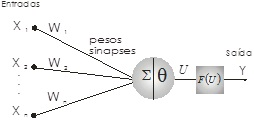
\includegraphics{modelomcp}
			\label{fig:modelomcp}
			\caption{Modelo MCP}
		\end{figure}
	\end{itemize}

	\item Funções de ativação

	\begin{itemize}
		\item Gera a saída $\gamma$ a partir dos pesos $\mathbf{w} = \{w_1, w_2, ..., w_n\}^T$ e da entrada $\mathbf{x} = \{x_1, x_2, ..., x_n\}^T$.
		\item Para o neurônio MCP, sua definição é:
		$$ f(u) = 			
			\begin{cases*}
			1 & $\sum_{i=1}^{n} x_i w_i \geq \theta $ \\
			0 & $\sum_{i=1}^{n} x_i w_i < \theta $
			\end{cases*}
		 $$
		 \begin{itemize}
		 	\item Onde $\theta$ é o limiar da função:
		 	$$ f(u) = \frac{1}{1+e^-{\beta u}}$$
		 	\item e $\beta$ é a inclinação da função.
		 \end{itemize}
		 \item Existem ainda funções de ativação sigmoidal, linear e gaussiana.
	\end{itemize}

	\item Arquiteturas de RNAs

	\begin{itemize}
		\item \textbf{Rede \textit{feedfoward} de uma única camada} - capaz de resolver problemas multivariáveis de múltiplas funções acopladas, com restrições de complexidade
		\item \textbf{Rede \textit{feedfoward} de duas camadas} - a camada intermediária dá uma maior capacidade computacional à rede e também universalidade na aproximação de funções contínuas.
		\item As duas primeiras são redes estáticas.
		\item \textbf{Rede com recorrência entre saídas e camada intermediária} - a saída depende também do valor atual, utilizada na resolução de problemas que envolvem processamento temporal.
		\item \textbf{Rede de recorrência auto-associativa} - possui um único nível de neurônios em que a saída de cada um está conectada às entradas de todos os outros. É uma estrutura típica de uma rede de Hopfield.
	\end{itemize}

	\item Aprendizado

	\begin{itemize}
		\item Na abordagem conexionista o conhecimento é adquirido através do ajuste das intensidades das conexões entre neurônios, e não através de regras explícitas, como em na IA simbólica.
		\item Portanto, aprendizado é o processo pelo qual os parâmetros livres de uma rede neural são ajustados por meio de uma forma continuada de estímulo do ambiente externo.
		\item O vetor de pessos $\mathbf{w}(t+1)$ é definido por 
		$$\mathbf{w}(t+1) = \mathbf{w}(t) + \Delta\mathbf{w}(t)$$
		\item Os algoritmos de aprendizado se diferem basicamente na forma como calculam $\Delta\mathbf{w}$.
	\end{itemize}

	\item Aprendizado supervisionado

	\begin{itemize}
		\item Há um \emph{supervisor} externo responsável por estimular as entradas da rede por meio de padrões de entrada e observar a saída calculada, comparando com a saída esperada.
		\item Se aplica a problemas em que se deseja obter um mapeamento entre padrões de entrada e saída.
		\item Na \textbf{correção de erros}, procura-se minimizar o erro da resposta atual em relação à saída desejada iterativamente.
		\item No \textbf{aprendizado por reforço}, um \emph{crítico} externo maximiza o reforço das ações boas executadas pela rede. É um processo de tentativa e erro que visa maximizar o índice de desempenho escalar.
	\end{itemize}

	\item Aprendizado não-supervisionado

	\begin{itemize}
		\item Não há o papel do \emph{supervisor}. No processo de aprendizado, a rede procura por regularidade e redundância nas entradas.
		\item Se aplica a problemas que visam à descoberta de características relevantes nos dados de entrada, como a descoberta de agrupamentos ou classes.
		\item O \textbf{Aprendizado Hebbiano} propõe que o peso de uma conexão sináptica deve ser ajustado se houver sincronismo entre os níveis de atividade da entrada e saída, isso é, se dois neurônios são ativados sincronamente, a sinapse entre eles é fortalecida, caso contrário enfraquecida ou mesmo eliminida.
		\item No \textbf{Aprendizado por competição} é ideia é, dado um padrão de entrada, fazer com que as unidades de saída disputem entre si para serem ativadas. 
	\end{itemize}

	\item Aplicações

	\begin{itemize}
		\item \textbf{Classificação} - atribuir um padrão desconhecido entre várias classes conhecidas. Normalmente redes com aprendizado supervisionado.
		\item \textbf{Categorização} - descoberta de categorias ou classes bem definidas nos dados de entrada. As classes não são conhecidas de antemão. Normalmente, aprendizado não supervisionado.
		\item \textbf{Aproximação} - mapear funções contínuas das variáveis de entrada.
		\item \textbf{Previsão} - estimativa de situações futuras com base nos estados atuais e anteriores do sistema a ser modelado.
		\item \textbf{Otimização} - podem ser resolvidos através de modelos recorrentes como as redes de Hopfield, os valores dos pesos são obtidos diretamente da formulação analítica do problema.
	\end{itemize}

\end{itemize}

\section{Perceptron}

\begin{itemize}
	\item Portas de Limiar
	\begin{itemize}
		\item Função: comparação da soma ponderada das entradas com um valor de limiar - \textit{threshold}
		\item Podem ser: Linear, Quadrática, Polinomial
		\item Porta de Limiar Linear
		\begin{itemize}
			\item Entradas são variáveis booleanas
			\item Solução de problemas que sejam linearmente separáveis, i.e., problemas cuja solução possar ser obtida pela separação de duas regiões por meio de uma reta
			\item Implementa soluções para funções \textbf{E}, \textbf{OU}, \textbf{NÃO-E} e \textbf{NÃO-OU}, mas não implementa solução para \textbf{OU-EXCLUSIVO}.
		\end{itemize}
		\item Porta de Limiar Quadrática
		\begin{itemize}
			\item Aumenta a capacidade computacional devido ao termo quadrático
			\item A equação da superfície de decisão resultante pode assumir uma forma não-linear
			\item Maior número de parâmetros livres
			\item Implementa função lógica \textbf{OU}
		\end{itemize}		
		\item \emph{Dilema entre a polarização e a variância}: uma rede com um número muito reduzido de parâmetros pode não possuir a flexibilidade necessária para alcançar a solução desejada; por outro lado, uma rede com um número muito grande de parâmetros pode estar superdimensiodada e, consequentemente, ser excessivamente flexível.
	\end{itemize}
	\item Perceptron
	\begin{itemize}
		\item Composto por uma estrutura de rede, tendo como unidades básicas neurônios MCP, e por uma regra de aprendizado.
		\item Um neurônio MCP treinado pelo algoritmo de aprendizado do Perceptron sempre converge caso o problema em questão seja linearmente separável
		\item Na topologia original, possuía uma unidade de entrada (retina), um nível intermediário formado pelas unidades de associação e um nível de saída formado pelas unidades de resposta. Conhecida como perceptron de uma única camada, pois só o nível de saída possui propriedades adaptativas.
		\item De uma maneira geral, durante o processo de aprendizado deseja-se obter no instante $n$, o valor do incremento $\Delta \mathbf{w}(n)$ aplicado ao vetor de pesos $\mathbf{w}(n)$ de tal forma que $\mathbf{w}(n+1) = \mathbf{w}(n) + \mathbf{w}(n)$ esteja mais próximo da solução desejada do que $\mathbf{w}(n)$.
		\item Equação geral para atualização dos pesos de um neurônio de um perceptron simples:
		$$ \mathbf{w}(n+1) = \mathbf{w}(n) + \eta e \mathbf{x}(n)$$
		\begin{itemize}
			\item $\eta$ é uma medida da rapidez com que o vetor de pesos será atualizado, ou \textit{taxa de aprendizado}.
			\item $e = y_d - y$, sendo $y_d$ o valor desejado e $y$ o saída obtida da rede
		\end{itemize}
		\item Algoritmo:
		\begin{enumerate}
			\item Inicializar $\eta$
			\item Inicializar o vetor de pesos $\mathbf{w}$ com valores aleatórios
			\item Aplicar a regra de atualização (equação geral) para todos os pares ($x^i,y_d^i$) do conjunto de treinamento
			\item Repetir o passo 3 até que $e = 0$ para todos os elementos do conjunto de treinamento
		\end{enumerate}
		\item Considerações sobre o algoritmo:
		\begin{itemize}
			\item O valor de $\eta$ deve ser definido pelo usuário, dependendo do problema em questão. Existem algoritmos que fazem o ajuste adaptativo de $\eta$
			\item Recomenda-se iniciar o vetor de pesos com valores amostrados em uma distribuição uniforme definida no intervalo $[-a,a]$, onde $a$ é um valor positivo próximo de $0.0$, como $0.5$, isso evita saturação forte do neurônio MCP, facilitando a convergência do algoritmo.
			\item Os pares de entrada e saída devem ser amostrados aleatoriamente.
		\end{itemize}
		\item Por fim, o Perceptron Simples é um discriminador que divide o espaço de entrada em duas regiões por meio de uma superfície de separação linear.
		\item Perceptron é uma rede neural simples para resolução de problemas de classificação.
	\end{itemize}

\end{itemize}

\section{Adaline}

	\begin{itemize}
		\item Como o perceptron, baseia-se em elementos de processamento que fazem operações sobre a soma ponderada de suas entradas.
		\item Diferentemente do perceptron, que usa funções degrau; no Adaline, essas operações são puramente lineares.
		\item Baseia-se na magnitude e no sinal do gradiente do erro para obter a direção e o valor do ajuste $\Delta \mathbf{w}$ aplicado ao vetor de pesos.		
		\item A equação do modelo é o produto entre os vetores $\mathbf{w}$ e $\mathbf{x}$:
		$$ y = f(\mathbf{x}, \mathbf{w}) = \mathbf{x} \cdot \mathbf{w} = \mathbf{x}^T \mathbf{w} = \sum_{i=0}^{n} x_i w_i$$
		$$ y = w_0 + w_1 x_1 + w_2 x_2 + ... + w_n x_n $$
		\begin{itemize}
			\item $w_0 = \theta$ é o termo de polarização
			\item $w_i$ são resultado do treinamento
		\end{itemize}
		\item Enquanto perceptron se caracteriza como separador linear, Adaline é um aproximador linear de funções. Perceptron resolve problemas de classificação de padrões e Adaline problemas aproximação de funções.
		\item Equação quadrática de erro
		$$ e^2 = (y_d^i)^2 - 2y_d^i(\mathbf{x} \cdot \mathbf{x}^i)+(\mathbf{w} \cdot \mathbf{x}^i)^2$$
		\begin{itemize}
			\item A equação é uma superfície na forma de parábola, que pode possuir um mínimo global.
			\item O objetivo do treinamento é atingir as regiões de menor erro, próximas ao mínimo global.
			\item A equação acima representa o erro para um par de treinamento, $\mathbf{x}^i$, $y_d^i$, para todos os padrões do conjunto de treinamento a equação é, chamada função de custo:
			$$ J = \frac{1}{2} \sum_{i=1}^{n} (y_d - (\mathbf{w} \cdot \mathbf{x^i}))^2$$
		\end{itemize}		
		\item Regra Delta
		\begin{itemize}
			\item O objetivo do treinamento é minimizar a função de custo J.
			\item A direção do ajuste na iteração $n$ pode ser obtida pelo gradiente da função de custo no ponto $\mathbf{w}(n)$.
			\item O ajuste dos pesos é então obtido por $\Delta \mathbf{w}(n) \propto - \nabla J$, expresso por:
			$$ \mathbf{w}(n+1) = \mathbf{w}(n)+\eta e \mathbf{x}(n) $$
		\end{itemize}
		\item Adaline também pode ser usado para fazer aproximação de combinação linear de funções, por exemplo: $f(x) = f_1(x) + f_2(x) + f_3(x) = sen(x) + cos(x) + x$
		\item Por fim, Perpcetron e Adaline são modelos de natureza simples e resolvem apenas problemas com características lineares. No entanto, é possível resolver problemas de natureza mais complexa com eles através da utilização de portas de limiar de maior complexidade ou através da combinação de funções não-lineares.
	\end{itemize}

\section{Perceptron de Múltiplas Camadas}

	\begin{itemize}
		\item As não-linearidades são incorporadas a modelos neurais através das funções de ativação (não-lineares) de cada neurônio da rede e da composição da sua estrutura em camadas sucessivas. Assim, a resposta da camada mais externa da rede corresponde à composição das respostas dos neurônios das camadas anteriores.
		\item Perceptron de Múltiplas Camadas (MLP) é a rede neural de múltiplas camadas composta por neurônios com funções de ativação 
		sigmoidais nas camadas intermediárias.
		\item Redes MLP apresentam um poder computacional maior do que aquele apresentado pelas redes de uma única camada.
		\item Para redes de múltiplas camadas, o erro $e$ só pode ser obtido a partir da última camada (única com saída), portanto, o problema passa a ser como calcular ou estimar o erro das camadas intermediárias.
		\item A solução é dada pelo algoritmo de \textit{back-propagation} - que utiliza o gradiente descendente para estimar o erro das camadas intermediárias por meio de uma estimativa do efeito que elas causam no erro da camada de saída. Assim, o erro na saída é calculado e este é retroalimentado para as camadas intermediárias, possibilitando o ajuste dos pesos proporcionalmente aos valores das conexões entre camadas.
		\item Por usar gradiente descendente, são necessárias aqui funções diferenciáveis, como as sigmoidais.
		\item O papel das múltiplas camadas é transformar sucessivamente o problema descrito pelo conjunto de dados no espaço de entrada em uma representação tratável para a camada de saída da rede. 
		\item Assim, por exemplo, um problema não-linearmente separável, resolvido por uma rede de duas camadas, é transformado em um problema linearmente separável pela camada intermediária, criando uma nova disposição interna à rede para os dados de entrada. A camada de saída pode então resolver o problema a partir dessa nova disposição.
		\item O comportamento da uma rede MLP de duas camadas pode ser descrito por meio de duas transformações sucessivas, a primeira $H(\mathbf{x}, \mathbf{w}_H)$ e a outra $Y(H(\mathbf{x}, \mathbf{w}_H); \mathbf{w}_s)$. Onde $\mathbf{w}_H$ e $\mathbf{w}_s$ são os vetores de pesos das camadas escondida e de saída, respectivamente.
		\item Quando se segue da primeira camada intermediária em direção à camada de saída, as funções implementadas se tornam cada vez mais complexas. Para uma rede com pelo menos duas camadas intermediárias, por exemplo:
		\begin{itemize}
			\item Na primeira camada intermediária, cada neurônio contribui com retas para a formação da superfície no espaço de entrada;
			\item Na segunda camadas intermediária, cada neurônio combina as retas descritas pela primeira camada, formando regiões convexas, com número de lados definido pelo número de neurônios ligados a ela.
			\item Na camada de saída, cada neurônio forma regiões que são combinações das regiões convexas definidas pelos neurônios a ele conectados da camada anterior, formando regiões com formatos diversos.
		\end{itemize}
		\item Dado um número suficientemente grande de unidades intermediárias, é possível formar representações internas para qualquer conjunto de padrões de entrada.
		\item Uma camada intermediária é suficiente para aproximar qualquer função contínua, e duas camadas intermediárias são suficientes para aproximar qualquer função.
		\item Funções de ativação
		\begin{itemize}
			\item Pelo menos uma das camadas intermediárias deverá ter funções de ativação não-lineares. A utilização de funções puramente lineares em múltiplas camadas resultaria em uma rede de uma única camada, já que transformações lineares sucessivas podem ser descritas como uma única transformação linear.
			\item Normalmente, funções lineares na saída são utilizadas em problemas de aproximação de funções, e funções sigmoidais em problemas de classificação, apesar de essa não ser uma regra geral.
		\end{itemize}
		\item Número de neurônios
		\begin{itemize}
			\item O número de neurônios determina a capacidade da rede em resolver problemas de determinada complexidade, quanto maior o número de neurônios, maior a complexidade da rede e maior a sua abrangência em termos de soluções possíveis.
			\item A determinação do número de neurônios é o problema mais fundamental em aprendizado de redes neurais. Não há uma regra geral que determine de forma precisa esse número.
			\item O problema básico de dimensionamento envolve um ajuste entre a complexidade do modelo neural e a complexidade do problema a ser resolvido.
			\item De forma empírica, procura-se por uma rede de estrutura mínima que atenda aos requisitos de minimmização do erro quadrático do conjunto de treinamento.
			\item Considere uma rede MLP com $n$ entradas. Essa estrutura irá possuir $n_p$ pesos:
			$$ n_p = (n \cdot N_e + N_e) + (N_e \cdot m + n) $$
			\begin{itemize}
				\item $N_e$ e $m$ correspondem aos termos de polarização dos neurônios das camadas escondidas e da saída, respectivamente.
				\item $n$ e $m$ são inerentes ao problema, somente $N_e$ é um parâmetro que altera a estrutura e a complexidade da rede.
				\item Aumentar o número de neurônios na camada escondida $N_e$ causará um aumento linear no número total de parâmetros $n_p$ da rede.
				\item Duas redes $R_1$ e $R_2$ com números diferentes de parâmetros $n_{p1} > n_{p2}$ e $\Delta n_p = n_{p1} - n_{p2}$. 
				\item As soluções alcançadas por $R_1$ serão todas as descritas por $R_2$ mais aquelas proporcionadas pela diferença no número de parâmetros $\Delta n_p$.
				\item O aumento no número de parâmetros causará, portanto, aumento no número de soluções possíveis.
				\item Considerando-se somente o erro de treinamento como critério de seleção do modelo, quanto maior o número de neurônios na rede, maior será o número de soluções que atendem ao critério de minimização do erro. No entanto, as soluções que se aproximam da função geradora dos dados estão em um número restrito no espaço de soluções e não aumenta em quantidade com o aumento do número de parâmetros. Assim, quanto maior o número de parâmetros, mais difícil é, na verdade, a busca pelas soluções que se aproximam da função geradora dos dados.
				\item Portanto, o objetivo do treinamento de redes MLP é minimizar não somente o erro do conjunto de treinamento, mas também a estrutura ou complexidade da rede.
			\end{itemize}
		\end{itemize}
		\item Treinamento
		\begin{itemize}
			\item \textit{Back-propagation} é um algoritmo de treinamento de redes MLP supervisionado.
			\item Por meio de pares de entrada e saída ($\mathbf{x}$, $y_d$) e um mecanismo de correção de erros ajusta os pesos da rede.
			\item O treinamento ocorre em duas fases:
			\begin{itemize}
				\item A primeira, \textit{forward}, é utilizada para definir a saída da rede para um dado padrão de entrada
				\item A segunda, \textit{backward}, utiliza a saída desejada e a saída da rede para atualizar os pesos de suas conexões, baseando-se na mesma Regra Delta usada pelo Adaline.
			\end{itemize}
			\item Etapa \textit{forward}:
			\begin{enumerate}
				\item O vetor de entrada $\mathbf{x}$ é apresentado às entradas da Rede e as saídas dos neurônios da primeira camada $C_1$ escondida é calculada
				\item As saídas da camada esconsida $C_1$ proverão as entradas da camada seguinte $C_2$. As saídas dessa camada são calculadas e o processo se repete até que se chegue à camada de saída $C_k$.
				\item As saídas produzidas pelos neurônios da camada de saída são então comparadas às saídas desejadas $y_d$ para o vetor de entrada $\mathbf{x}$, e o erro correspondente é calculado.
			\end{enumerate}
			\item Etapa \textit{backward}:
			\begin{enumerate}
				\item O erro da camada de saída $C_k$ é usado para ajustar seus pesos utilizando o gradiente descendente do erro.
				\item Os erros dos neurônios da camada $C_k$ são propagados para a camada anterior $C_{k-1}$, utlizando-se os pesos das conexões entre as camadas, que são multiplicados pelos erros correspondentes. Obtendo-se um valor de erro estimado para cada neurônio da camada escondida.
				\item Os erros calculados para a camada $C_{k-1}$ são então utilizados para ajustar os seus pesos pelo gradiente descendente.
				\item O processo se repete até que os pesos da camada $C_1$ sejam ajustados.
			\end{enumerate}			
			\item O ajuste dos pesos na camada de saída é dado por:
			$$ \Delta w_{ij} = \alpha e_j(n)f'(u_j(n))h_i(n)$$
			\begin{itemize}
				\item $i$ é o índice do neurônio da camada escondida
				\item $j$ é o índice dos neurônios da camada de saída
				\item $e_j(n)$ é o erro apresentado na saída para a entrada $n$
				\item $h_i(n)$ é a saída do $i$-ésimo neurônio da camada escondida
				\item $u(n)$ é o somatório das saídas da camada escondida ponderada pelos pesos $w_{jk}$
				\item $f'$ é a derivada da função de ativação da camada de saída
				\item $\alpha$ é a taxa de aprendizado
			\end{itemize}
			\item Para a camada de saída, a equação é:
			$$ \Delta w_{jk} = \eta h'_i(u_i(n)) \sum_j e_j(n) f'(u_j(n))w_{ji}x_k(n)$$
			\begin{itemize}
				\item $k$ é o índice da entrada $x$
				\item $h'$ é a derivada da função de ativação da camada escondida
				\item $\eta$ é a taxa de aprendizado
			\end{itemize}
		\end{itemize}				
	\end{itemize}
\end{document}

